


\section{Experiments}


\subsection{Experiments Setting}

\noindent\textbf{Environment}. Following the standard evaluation protocol adopted in prior studies \cite{lifshitz2024steve,wang2023describe,wang2023jarvis,qin2023mp5,li2024optimus}, we conduct experiments in the open-world environment of Minecraft on the MineRL \cite{guss2019minerl} platform. It is an archetypal open-world environment that offers rich diversity in resources and biomes, thereby requiring agents to operate under long-horizon and highly variable conditions. In MineRL, the agent receives instructions and observations then produces mouse/keyboard control actions at 20 Hz. For each episode, the agent is spawned without any initial equipment and is initialized at random biomes and positions, leading to substantial variation in environmental dynamics and task difficulty. Therefore, Minecraft serves as a suitable and challenging testbed for evaluating open-world agents.
\begin{table}[ht]
\centering
\caption{Hyperparameter setting for each training phase.}
\label{tab:hyper}
\resizebox{0.45\textwidth}{!}{%
\renewcommand\arraystretch{1.2}
\begin{tabular}{lccc}
\toprule[1.2pt]
Hyperparameter & Stage-1 & Stage-2 & Stage-3 \\ \hline
Optimizer      & AdamW   & AdamW      & AdamW       \\
Learning Rate  & 5.0e-5   & 3.0e-5   & 1.0e-6     \\
Epochs         & 2     & 2       & 20           \\
Batch Size      & 12    & 8    & 16        \\
Gradient Accumulation & 16 & 16 & 8 \\
Warm Up Ratio & 0.25 & 0.25 & - \\
Max Pixels & 234416 & 234416 & 234416 \\
Num Generations & - & - & 5 \\
Max Prompt Length & 2048 & 2048 & 2048 \\
\bottomrule[1.2pt]
\end{tabular}
}
\end{table}

\noindent\textbf{Implementation details}. We initialize Optimus-3 with the weights of Qwen2.5-VL-7B \cite{bai2025qwen2}. It comprises a large language model (LLM) and a ViT-based \cite{dosovitskiy2020vit} visual encoder. Then we adapt it into MoE architecture, comprising one shared knowledge expert and five task-specific experts dedicated to planning, perception, action, grounding, and reflection. Subsequently, we implement the Task Router by fine-tuning a lightweight Sentence-BERT \cite{reimers2019sentence} model to classify instructions into the predefined task set. For Action tasks, following prior work \cite{li2025optimus}, we employ  VPT \cite{vpt} as action head to generate low-level actions. We collect 230k samples for training stage-1, 58k samples for the training stage-2, and 5k samples for training stage-3. These datasets are sourced from our proposed OptimusM$^4$ as well as previous works \cite{vpt,li2025optimus,qin2023mp5}. All experiments were conducted on 8$\times$ NVIDIA L40 GPUs. The hyperparameter setting are shown in Table \ref{tab:hyper}.
% PleAS $\downarrow$e add the following required packages to your document preamble:
% \usepackage{multirow}
% \usepackage{graphicx}

\begin{table*}[t]
\scriptsize
\centering
\caption{Evaluation Results of Optimus-3 on MineSys2 benchmark. \#Params denotes activated parameters. SFT and RL refer to supervised fine-tuning and reinforcement learning, respectively.}
\label{tb:main_text}
\renewcommand\arraystretch{1.1}
\resizebox{0.8\textwidth}{!}{%

\begin{tabular}{lcccccc}
\toprule[1.2pt]
\multirow{2}{*}{Model} & \multirow{2}{*}{\#Params} & Planning & Captioning & EQA & Grounding & Reflection \\
      &          & \texttt{Acc}      & \texttt{Score}      & \texttt{Score} & \texttt{IoU@0.5}  & \texttt{Acc} \\
\hline
\multicolumn{7}{c}{\textit{Generalist Multimodal Large Language Model}} \\
\hline
GPT-4o   \cite{gpt4}       &   \multicolumn{1}{c}{-}  &  0.20   &   0.46  & 0.33   &  -  & 0.31   \\
Gemini-1.5-pro  \cite{team2024gemini}      &    \multicolumn{1}{c}{-} &   0.19   & 0.33    & 0.33   & -   &  0.34    \\
DeepSeek-VL2 \cite{lu2024deepseek}        &   4B  &   0.07   &  0.49  &   0.51  &  0.29  &  0.47  \\
Qwen2.5-VL \cite{bai2025qwen2}          &   3B  &  0.03    & 0.37    & 0.40   &  0.58  & 0.47   \\
Qwen2.5-VL \cite{bai2025qwen2}          &   7B  &   0.05   &  0.47  &   0.46  &  0.18  &  0.56  \\
Qwen2.5-VL \cite{bai2025qwen2}          &   32B  &  0.07    & 0.51    & 0.49   &  0.34  & 0.53   \\
Qwen2.5-VL \cite{bai2025qwen2}          &   72B  &   0.09   &  0.52  &   0.54  &  0.32  &  0.53  \\

\hline
\multicolumn{7}{c}{\textit{Post-trained Multimodal Large Language Model}} \\
\hline
Qwen2.5-VL-SFT \cite{bai2025qwen2}      &   3B    &   0.76  & 0.64  &  0.69 & 0.69   & 0.47     \\
Qwen2.5-VL-RL  \cite{bai2025qwen2}      &   3B   &     0.74 & 0.65    &  0.70  &  0.71  &  0.48    \\
Qwen2.5-VL-SFT  \cite{bai2025qwen2}     &   7B    &   0.79   & 0.68   &   0.71 &   0.52   & 0.53      \\
Qwen2.5-VL-RL  \cite{bai2025qwen2}      &   7B   &   0.76   & 0.71    &   0.68 &  0.79  & 0.56     \\ 

\hline
\rowcolor[HTML]{E7EEFE}
Optimus-3 $_{[token\;routing]}$            &    6.8B &  0.88   &   0.66  & 0.77   &  0.75  &  0.58    \\
\rowcolor[HTML]{E7EEFE}
Optimus-3 $_{[task\;routing]}$            &    6.8B &   \textbf{0.94}   &   \textbf{0.78}  & \textbf{0.81}   & \textbf{0.80}  &    \textbf{0.66}   \\
\bottomrule[1.2pt]
\end{tabular}
}
\end{table*}



%%%

\begin{table*}[htbp]
\centering
\caption{Main Result of Optimus-3 on Long-Horizon Benchmark. We report \texttt{SR} on each task group. ${\dagger}$ denotes we employ a hierarchical architecture agent from prior work \cite{li2025optimus}, where an MLLM serves as the planner, followed by STEVE-1 \cite{lifshitz2024steve} acting as the policy to sequentially generate actions. ${*}$ represents reproduced results under the same settings as other baselines. Optimus-3-Action denotes Optimus-3 trained only on action trajectories.}
\label{tb:main_horizon}
\scriptsize
\renewcommand\arraystretch{1.2}
\resizebox{1\textwidth}{!}{%
\begin{tabular}{lccccccc}
\toprule[1.2pt]
Method       & Wood 
\includegraphics[width=0.3cm]{figures/logo/wood.pdf} & Stone 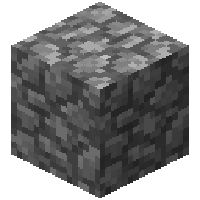
\includegraphics[width=0.3cm]{figures/logo/cobblestone.pdf} & Iron 
\includegraphics[width=0.3cm]{figures/logo/iron_ingot.pdf} & Gold 
\includegraphics[width=0.3cm]{figures/logo/gold_ingot.pdf} & Diamond 
\includegraphics[width=0.3cm]{figures/logo/diamond.pdf} & RedStone 
\includegraphics[width=0.3cm]{figures/logo/readstone.pdf} & Armor 
\includegraphics[width=0.3cm]{figures/logo/armor.pdf}  \\
\hline
\multicolumn{8}{c}{\textit{Multimodal Large Language Model$^{\dagger}$}} \\
\hline
 GPT-3.5 \cite{gpt3}      &    0.40$\scriptstyle\pm\,0.15$  &   0.20$\scriptstyle\pm\,0.13$    &   0.00$\scriptstyle\pm\,0.00$  &   0.00$\scriptstyle\pm\,0.00$   &     0.00$\scriptstyle\pm\,0.00$    &       0.00$\scriptstyle\pm\,0.00$   &    0.00$\scriptstyle\pm\,0.00$           \\
GPT-4o \cite{gpt4}    &    0.47$\scriptstyle\pm\,0.23$   &   0.23$\scriptstyle\pm\,0.09$    &   0.05$\scriptstyle\pm\,0.04$  &   0.00$\scriptstyle\pm\,0.00$   &     0.00$\scriptstyle\pm\,0.00$    &       0.00$\scriptstyle\pm\,0.00$   &    0.00$\scriptstyle\pm\,0.00$           \\
Gemini-1.5-pro \cite{team2024gemini}   &  0.41$\scriptstyle\pm\,0.14$    &  0.21$\scriptstyle\pm\,0.10$    & 0.03$\scriptstyle\pm\,0.02$    &   0.00$\scriptstyle\pm\,0.00$   &     0.00$\scriptstyle\pm\,0.00$    &       0.00$\scriptstyle\pm\,0.00$   &    0.00$\scriptstyle\pm\,0.00$           \\
Qwen2.5-VL \cite{bai2025qwen2}     &  0.28$\scriptstyle\pm\,0.15$    &   0.06$\scriptstyle\pm\,0.03$    &  0.00$\scriptstyle\pm\,0.00$   &   0.00$\scriptstyle\pm\,0.00$  &     0.00$\scriptstyle\pm\,0.00$    &       0.00$\scriptstyle\pm\,0.00$   &    0.00$\scriptstyle\pm\,0.00$           \\
Qwen2.5-VL-SFT \cite{bai2025qwen2}    &  0.76$\scriptstyle\pm\,0.11$    & 0.36$\scriptstyle\pm\,0.07$      &   0.11$\scriptstyle\pm\,0.05$  &  0.00$\scriptstyle\pm\,0.00$    &   0.00$\scriptstyle\pm\,0.00$     &     0.00$\scriptstyle\pm\,0.00$    &   0.00$\scriptstyle\pm\,0.00$          \\
\hline
\multicolumn{8}{c}{\textit{Goal-conditioned Policy in Minecraft}} \\
\hline
VPT \cite{vpt}   \texttt{[NeurIPS'22]}   &  0.18$\scriptstyle\pm\,0.15$   &  0.07$\scriptstyle\pm\,0.05$    &   0.00$\scriptstyle\pm\,0.00$   &  0.00$\scriptstyle\pm\,0.00$    &   0.01$\scriptstyle\pm\,0.01$      &   0.00$\scriptstyle\pm\,0.00$       &   0.00$\scriptstyle\pm\,0.00$           \\
GROOT \cite{cai2023groot}   \texttt{[ICLR'24]}      &  0.34$\scriptstyle\pm\,0.17$   &  0.17$\scriptstyle\pm\,0.10$    &   0.08$\scriptstyle\pm\,0.05$   &  0.01$\scriptstyle\pm\,0.01$    &   0.01$\scriptstyle\pm\,0.01$      &   0.03$\scriptstyle\pm\,0.02$       &   0.04$\scriptstyle\pm\,0.02$           \\
MineCLIP \cite{fan2022minedojo}  \texttt{[NeurIPS'22]}      &  0.23$\scriptstyle\pm\,0.16$   &  0.12$\scriptstyle\pm\,0.08$    &   0.06$\scriptstyle\pm\,0.05$   &  0.00$\scriptstyle\pm\,0.00$    &   0.00$\scriptstyle\pm\,0.00$      &   0.00$\scriptstyle\pm\,0.00$       &   0.02$\scriptstyle\pm\,0.02$           \\
STEVE-1 \cite{lifshitz2024steve}    \texttt{[NeurIPS'23]}     &  0.45$\scriptstyle\pm\,0.22$   &  0.22$\scriptstyle\pm\,0.19$    &   0.08$\scriptstyle\pm\,0.06$   &  0.00$\scriptstyle\pm\,0.00$    &   0.05$\scriptstyle\pm\,0.03$      &   0.00$\scriptstyle\pm\,0.00$       &   0.07$\scriptstyle\pm\,0.05$           \\

\hline
\multicolumn{8}{c}{\textit{Agents in Minecraft}} \\
\hline
Voyager$^{*}$ \cite{wang2023describe}    \texttt{[NeurIPS'23]}    &  0.87$\scriptstyle\pm\,0.25$   &  0.32$\scriptstyle\pm\,0.15$    &   0.08$\scriptstyle\pm\,0.06$   &  0.02$\scriptstyle\pm\,0.02$    &   0.01$\scriptstyle\pm\,0.01$      &   0.00$\scriptstyle\pm\,0.00$       &   0.14$\scriptstyle\pm\,0.09$           \\
DEPS \cite{wang2023describe}    \texttt{[NeurIPS'23]}     &  0.77$\scriptstyle\pm\,0.13$   &  0.48$\scriptstyle\pm\,0.09$    &   0.16$\scriptstyle\pm\,0.08$   &  0.00$\scriptstyle\pm\,0.00$    &   0.01$\scriptstyle\pm\,0.01$      &   0.00$\scriptstyle\pm\,0.00$       &   0.10$\scriptstyle\pm\,0.18$           \\
MP5$^{*}$ \cite{qin2023mp5}    \texttt{[CVPR'24]}     &  0.89$\scriptstyle\pm\,0.23$   &  0.73$\scriptstyle\pm\,0.21$    &   0.43$\scriptstyle\pm\,0.18$   &  0.10$\scriptstyle\pm\,0.08$    &   0.09$\scriptstyle\pm\,0.08$      &   0.17$\scriptstyle\pm\,0.08$       &   0.19$\scriptstyle\pm\,0.18$           \\
JARVIS-1 \cite{wang2023jarvis}    \texttt{[TPAMI'25]}  &  0.93$\scriptstyle\pm\,0.14$   &    0.89$\scriptstyle\pm\,0.07$   &  0.36$\scriptstyle\pm\,0.06$    &  0.07$\scriptstyle\pm\,0.03$    &    0.08$\scriptstyle\pm\,0.03$    &     0.16$\scriptstyle\pm\,0.07$     &   0.15$\scriptstyle\pm\,0.19$            \\
Optimus-1 \cite{li2024optimus}  \texttt{[NeurIPS'24]}  &  0.98$\scriptstyle\pm\,0.02$   & 0.92$\scriptstyle\pm\,0.04$    & 0.46$\scriptstyle\pm\,0.09$    &   0.08$\scriptstyle\pm\,0.05$  &     0.11$\scriptstyle\pm\,0.05$   &   0.25$\scriptstyle\pm\,0.03$    &   0.19$\scriptstyle\pm\,0.22$          \\ 
Optimus-2 \cite{li2025optimus}   \texttt{[CVPR'25]}   & 0.99$\scriptstyle\pm\,0.02$   & 0.93$\scriptstyle\pm\,0.04$    & 0.53$\scriptstyle\pm\,0.03$   &   0.09$\scriptstyle\pm\,0.01$  &   0.13$\scriptstyle\pm\,0.02$    &    0.28$\scriptstyle\pm\,0.03$   &   0.21$\scriptstyle\pm\,0.19$   \\ 
\hline
\rowcolor[HTML]{E7EEFE}
Optimus-3-Action      &    0.93$\scriptstyle\pm\,0.03$ & 0.87$\scriptstyle\pm\,0.05$      &  0.49$\scriptstyle\pm\,0.04$   &  0.03$\scriptstyle\pm\,0.04$  &  0.03$\scriptstyle\pm\,0.02$      &   0.09$\scriptstyle\pm\,0.05$     &   0.15$\scriptstyle\pm\,0.22$  \\
\rowcolor[HTML]{E7EEFE}
Optimus-3      &    \textbf{0.99$\scriptstyle\pm\,0.01$} & \textbf{0.95$\scriptstyle\pm\,0.02$}      &  \textbf{0.55$\scriptstyle\pm\,0.03$}   &  \textbf{0.10$\scriptstyle\pm\,0.02$}  &  \textbf{0.15$\scriptstyle\pm\,0.02$}      &   \textbf{0.29$\scriptstyle\pm\,0.02$}     &   \textbf{0.23$\scriptstyle\pm\,0.16$}  \\


\bottomrule[1.2pt]
\end{tabular}
\vspace{-5pt}
}

\end{table*}




%%%




\subsection{Evaluation on System 2 Tasks}
\noindent\textbf{Evaluation Tasks \& Metrics}. To comprehensively evaluate the multi-dimensional cognitive abilities of Optimus-3, we construct a MineSys2 Benchmark comprising five categories: \textit{Planning}, \textit{Captioning}, \textit{Embodied QA}, \textit{Grounding}, and \textit{Reflection}. For \textit{Planning} and \textit{Reflection} tasks, evaluation samples are 103 and 64, respectively. We employ average accuracy (\texttt{Acc}) as the evaluation metric. For the \textit{Captioning} and \textit{Embodied QA} tasks, the evaluation includes 134 and 400 samples, respectively. We adopt an LLM-as-Judge \cite{li2024generation} approach, employing GPT-4 \cite{gpt4} to assign a score from 1 to 10 for each sample. The average score is then normalized to a value between 0 and 1. For the \textit{Grounding} tasks, we construct 500 evaluation samples, and use \texttt{IOU@0.5} \cite{chen2023advancing} as the metric.

\begin{table*}[t]
\centering

\caption{Performance comparison on Wooden Pickaxe 
\includegraphics[width=0.3cm]{figures/logo/wooden_pickaxe.pdf}, Stone Sword 
\includegraphics[width=0.3cm]{figures/logo/stone_sword.pdf}, Iron Ingot 
\includegraphics[width=0.3cm]{figures/logo/iron_ingot.pdf}, Golden Shovel 
\includegraphics[width=0.3cm]{figures/logo/Golden_Shovel.pdf}, and Diamond Sword 
\includegraphics[width=0.3cm]{figures/logo/diamond_sword.pdf}. We report Completion Rate (\texttt{CR}) and Success Rate (\texttt{SR}) for each task. ${\dagger}$ denotes we employ a hierarchical architecture agent from prior work \cite{li2025optimus}. ${*}$ represents reproduced results under the same settings. }
\label{tb:main_open}
\renewcommand\arraystretch{1.2}
 
\resizebox{1\textwidth}{!}{%

\begin{tabular}{lcccccccccccc}
\toprule[1.2pt]
\multirow{2}{*}{Model} & \multicolumn{2}{c}{Wooden Pickaxe 
\includegraphics[width=0.3cm]{figures/logo/wooden_pickaxe.pdf}} & \multicolumn{2}{c}{Stone Sword 
\includegraphics[width=0.3cm]{figures/logo/stone_sword.pdf}} & \multicolumn{2}{c}{Iron Ingot 
\includegraphics[width=0.3cm]{figures/logo/iron_ingot.pdf}} & \multicolumn{2}{c}{Golden Shovel 
\includegraphics[width=0.3cm]{figures/logo/Golden_Shovel.pdf}} & \multicolumn{2}{c}{Diamond Sword 
\includegraphics[width=0.3cm]{figures/logo/diamond_sword.pdf}} & \multicolumn{2}{c}{Avg} \\
\cmidrule(lr){2-3} \cmidrule(lr){4-5} \cmidrule(lr){6-7} \cmidrule(lr){8-9} \cmidrule(lr){10-11} \cmidrule(lr){12-13}
 & \texttt{CR} & \texttt{SR}  & \texttt{CR} & \texttt{SR}  & \texttt{CR} & \texttt{SR}  & \texttt{CR} & \texttt{SR}  & \texttt{CR} & \texttt{SR}  & \texttt{CR} & \texttt{SR} \\
\hline
\multicolumn{13}{c}{\textit{Multimodal Large Language Model$^{\dagger}$}} \\
\hline
GPT-5-Instant \cite{gpt5}             & 0.22 & 0.05 & 0.18 & 0.05 & 0.14 & 0.00 & 0.12 & 0.00 & 0.12 & 0.00 & 0.15 & 0.02 \\
GPT-5-Thinking \cite{gpt5}             & 0.28 & 0.10 & 0.24 & 0.05 & 0.16 & 0.00 & 0.14 & 0.00 & 0.12 & 0.00 & 0.18 & 0.03 \\
Gemini-2.5-Flash \cite{gemini2.5}     & 0.24 & 0.10 & 0.22 & 0.10 & 0.16 & 0.05 & 0.14 & 0.05 & 0.14 & 0.00 & 0.18 & 0.06 \\
Gemini-2.5-Pro \cite{gemini2.5}     & 0.36 & 0.25 & 0.30 & 0.20 & 0.28 & 0.10 & 0.22 & 0.05 & 0.14 & 0.00 & 0.26 & 0.12 \\
Qwen2.5-VL-7B \cite{bai2025qwen2}   & 0.31 & 0.20 & 0.26 & 0.20 & 0.24 & 0.10 & 0.19 & 0.05 & 0.09 & 0.00 & 0.21 & 0.11 \\
\hline
\multicolumn{13}{c}{\textit{Agents in Minecraft}} \\
\hline
Voyager$^{*}$ \cite{wang2023voyager} \texttt{[NeurIPS'23]}   & 0.16 & 0.10 & 0.16 & 0.05 & 0.14 & 0.00 & 0.14 & 0.00 & 0.08 & 0.00 & 0.14 & 0.03 \\
DEPS$^{*}$ \cite{wang2023describe} \texttt{[NeurIPS'23]}   & 0.14 & 0.10 & 0.14 & 0.10 & 0.12 & 0.05 & 0.12 & 0.00 & 0.10 & 0.05 & 0.12 & 0.06 \\
MP5$^{*}$ \cite{qin2023mp5}  \texttt{[CVPR'24]}  & 0.29 & 0.20 & 0.19 & 0.20 & 0.18 & 0.15 & 0.18 & 0.05 & 0.16 & 0.10 & 0.20 & 0.14 \\
Jarvis-1$^{*}$ \cite{wang2023jarvis} \texttt{[TPAMI'25]}   & 0.19 & 0.15 & 0.18 & 0.15 & 0.18 & 0.10 & 0.20 & 0.10 & 0.12 & 0.05 & 0.17 & 0.11 \\
Optimus-1$^{*}$ \cite{li2024optimus} \texttt{[NeurIPS'24]}   & 0.21 & 0.20 & 0.18 & 0.20 & 0.18 & 0.15 & 0.17 & 0.15 & 0.12 & 0.10 & 0.17 & 0.16 \\
Optimus-2$^{*}$ \cite{li2025optimus}  \texttt{[CVPR'25]}   & 0.22 & 0.25 & 0.21 & 0.15 & 0.18 & 0.15 & 0.19 & 0.10 & 0.19 & 0.15 & 0.19 & 0.16 \\
\hline
\rowcolor[HTML]{E7EEFE}
Optimus-3           & 
\textbf{0.89} & \textbf{0.75} & \textbf{0.86} & \textbf{0.70} & \textbf{0.79} & \textbf{0.65} & \textbf{0.75} & \textbf{0.55} & \textbf{0.69} & \textbf{0.35} & \textbf{0.79} & \textbf{0.60} \\
\bottomrule[1.2pt]
\end{tabular}
}
\end{table*}
\noindent\textbf{Baselines}. For the MineSys2 Benchmark, we compare Optimus-3 against generalist MLLMs (GPT-4o \cite{gpt4}, Qwen2.5-VL \cite{bai2025qwen2}, Gemini-1.5-pro \cite{team2024gemini}), and various variants of Qwen2.5-VL \cite{bai2025qwen2} that post-trained on OptimusM$^4$ dataset.



\noindent\textbf{Results Analysis}.  As depicted in Table \ref{tb:main_text}, compared to all baselines, Optimus-3 achieves the highest performance across all System 2 tasks. The first four rows of Table \ref{tb:main_text} reveal the limited capabilities of existing generalist MLLMs, due to the fact that they have not been post-trained in the Minecraft domain. In contrast, \texttt{Qwen2.5-VL-SFT}, which post-trained on OptimusM$^4$, shows a notable performance boost. Furthermore, after applying our proposed DGRPO method, \texttt{Qwen2.5-VL-RL} achieves a 52\% improvement in \textit{Grounding}. More importantly, we observe that the various variants of Qwen2.5-VL exhibit task interference, while Optimus-3 consistently achieves superior performance across tasks. Moreover, compared to token-level routing, the proposed task-level routing demonstrates superior performance on tasks such as \textit{Captioning}, \textit{Planning}, and \textit{Grounding}. We attribute this improvement to the Dual-route Aligned MoE architecture in Optimus-3, which allocates task-specific experts via task router, thereby effectively mitigating conflicts among heterogeneous tasks. 

\begin{figure}[t]
\centering
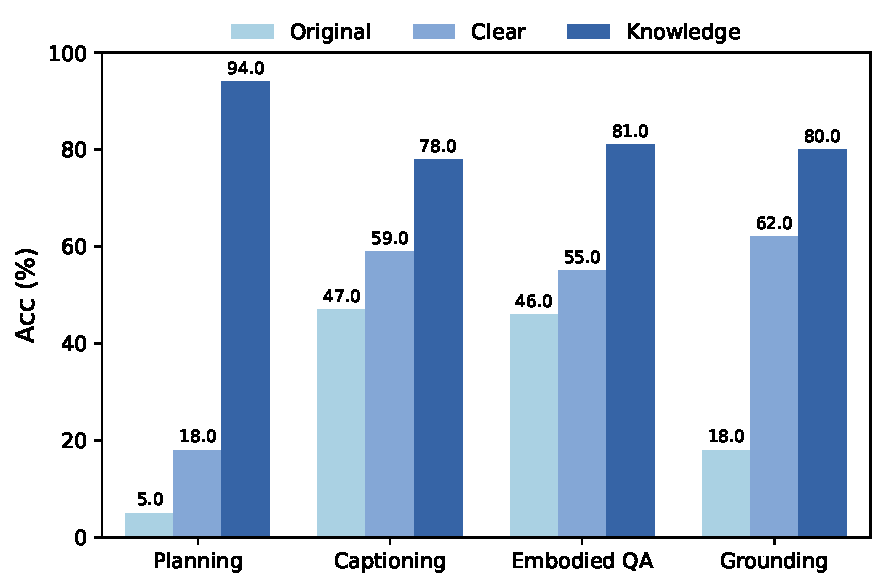
\includegraphics[width=0.45\textwidth]{figures/fig8.pdf}
\caption{Ablation Study on Training Data. \texttt{Original} refers to the original Qwen2.5-VL-7B, \texttt{Clear} indicates the Optimus-3 post-trained on data without knowledge, \texttt{Knowledge} represents the Optimus-3 post-trained on OptimusM$^4$.}
\label{fig:fig8}
\end{figure}

\subsection{Evaluation on System 1 Tasks}
\noindent\textbf{Evaluation Tasks \& Metrics}. To evaluate the robustness of Optimus-3 in executing long-horizon action sequences, we follow the experimental setup of prior work and conduct experiments on the Long-Horizon benchmark \cite{li2024optimus}. It comprises 67 tasks spanning 7 technology groups: Wooden (10 tasks), Stone (9 tasks), Iron (16 tasks), Gold (6 tasks), Diamond (7 tasks), Redstone (6 tasks), and Armor (13 tasks). Each task consists of multiple sub-steps that the agent must execute sequentially to reach the final goal. For each task, we perform at least 30 rollouts from different initial positions, and we report the average Success Rate (\texttt{SR}) with standard deviation on each task group as the evaluation metric.

\noindent\textbf{Baselines}. We follow the hierarchical architecture of agents from prior work, employing an MLLM (GPT-3.5 \cite{gpt3}, GPT-4o \cite{gpt4}, Qwen2.5-VL\cite{bai2025qwen2}, Gemini-1.5-pro \cite{team2024gemini}) as a planner to generate sub-goals, followed by STEVE-1 as a policy to sequentially generate actions. Moreover, we employ current SOTA agents in Minecraft (DEPS \cite{wang2023describe}, Jarvis-1 \cite{wang2023jarvis}, Optimus-1 \cite{li2024optimus}, and Optimus-2 \cite{li2025optimus}) as baselines.


\begin{figure}[t]
\centering
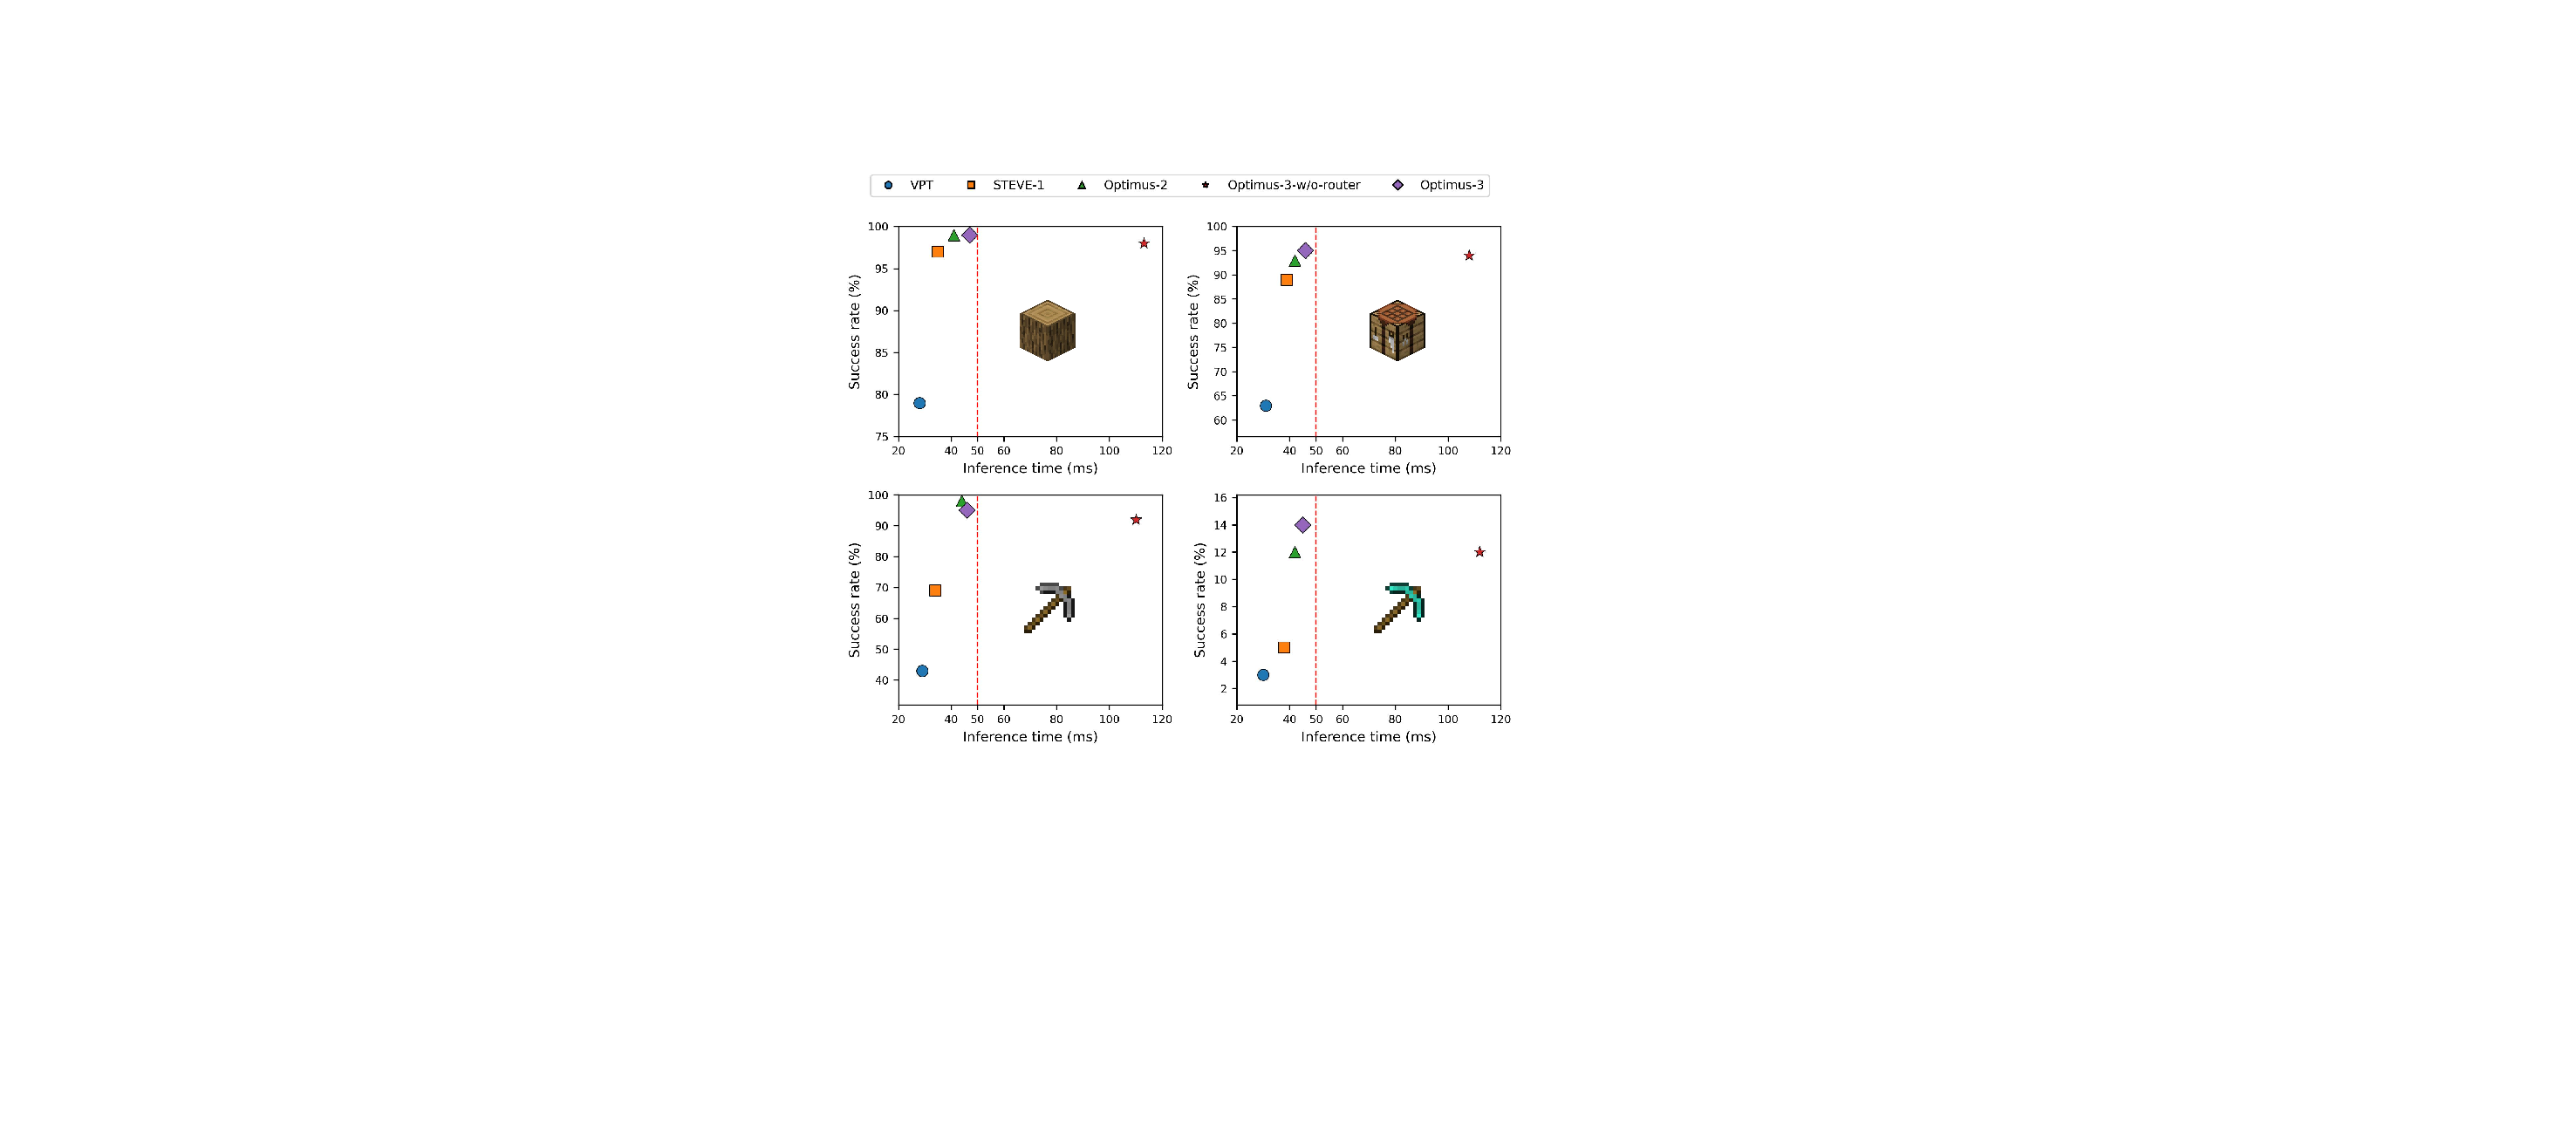
\includegraphics[width=0.4\textwidth]{figures/fig9.pdf}
\caption{Comparison of the average per-action inference time on Log 
\includegraphics[width=0.3cm]{figures/logo/wood.pdf}, Crafting Table 
\includegraphics[width=0.3cm]{figures/logo/crafting_table.pdf}, Stone Pickaxe 
\includegraphics[width=0.3cm]{figures/logo/stone_pickaxe.pdf}, and Diamond Pickaxe 
\includegraphics[width=0.3cm]{figures/logo/diamond_pickaxe.pdf}. \texttt{Optimus-3-w/o-router} denotes the variant of Optimus-3 without Layer Router. The 50\,ms mark corresponds to Minecraft's real-time interaction requirement, i.e., 20\,Hz.}
\label{fig:fig9}
\end{figure}
\noindent\textbf{Results Analysis}. As shown in Table \ref{tb:main_horizon}, Optimus-3 achieves the highest success rate across all 7 task groups, with particularly strong performance on the Diamond Group, attaining a \texttt{SR} of 15\%. It is worth emphasizing that Optimus-3 performs both high-level planning and low-level action execution within an end-to-end architecture, whereas all baseline agents \cite{wang2023describe,wang2023jarvis,li2024optimus,li2025optimus} rely on additional external tools or task-specific modules to bridge these two stages. The results in Rows 1-4 of Table~\ref{tb:main_horizon} show that generic MLLMs struggle to produce effective long-horizon plans, which we attribute to the absence of domain-specific fine-tuning in Minecraft. In contrast, \texttt{Qwen2.5-VL-SFT} is fine-tuned on our proposed OptimusM$^4$ dataset, its planning capability improves substantially. It highlights the critical role of OptimusM$^4$ in injecting Minecraft-specific knowledge and structured long-horizon planning skills. Moreover, compared with the variant (\texttt{Optimus-3-Action}) trained solely on action-trajectory data, Optimus-3 trained on a diverse set of task types achieves a substantially higher success rate. We attribute this improvement to the richer domain knowledge contained in the different task families, which enhances the model's representations. While shared knowledge expert in Optimus-3 enables such knowledge transfer across tasks.



\subsection{Evaluation on Open-ended Tasks}

\noindent\textbf{Evaluation Tasks \& Metrics}. To evaluate the performance of Optimus-3 to jointly deploy its diverse capabilities in open-ended scenarios, we construct a suite of five open-ended tasks corresponding to the Wooden, Stone, Iron, Gold, and Diamond tech levels. For each episode, the agent is randomly initialized at a different location, and endowed with a set of initial resources sampled from a predefined resource pool. This setup requires the agent to leverage its multi-dimensional abilities, e.g.,  perception, planning, and reflection, to make adaptive decisions conditioned on the current state. For each task, we perform 20 rollouts and employ the average Success Rate (\texttt{SR}) and average Completion Rate (\texttt{CR}) as evaluation metrics. \begin{figure*}[t]
\centering
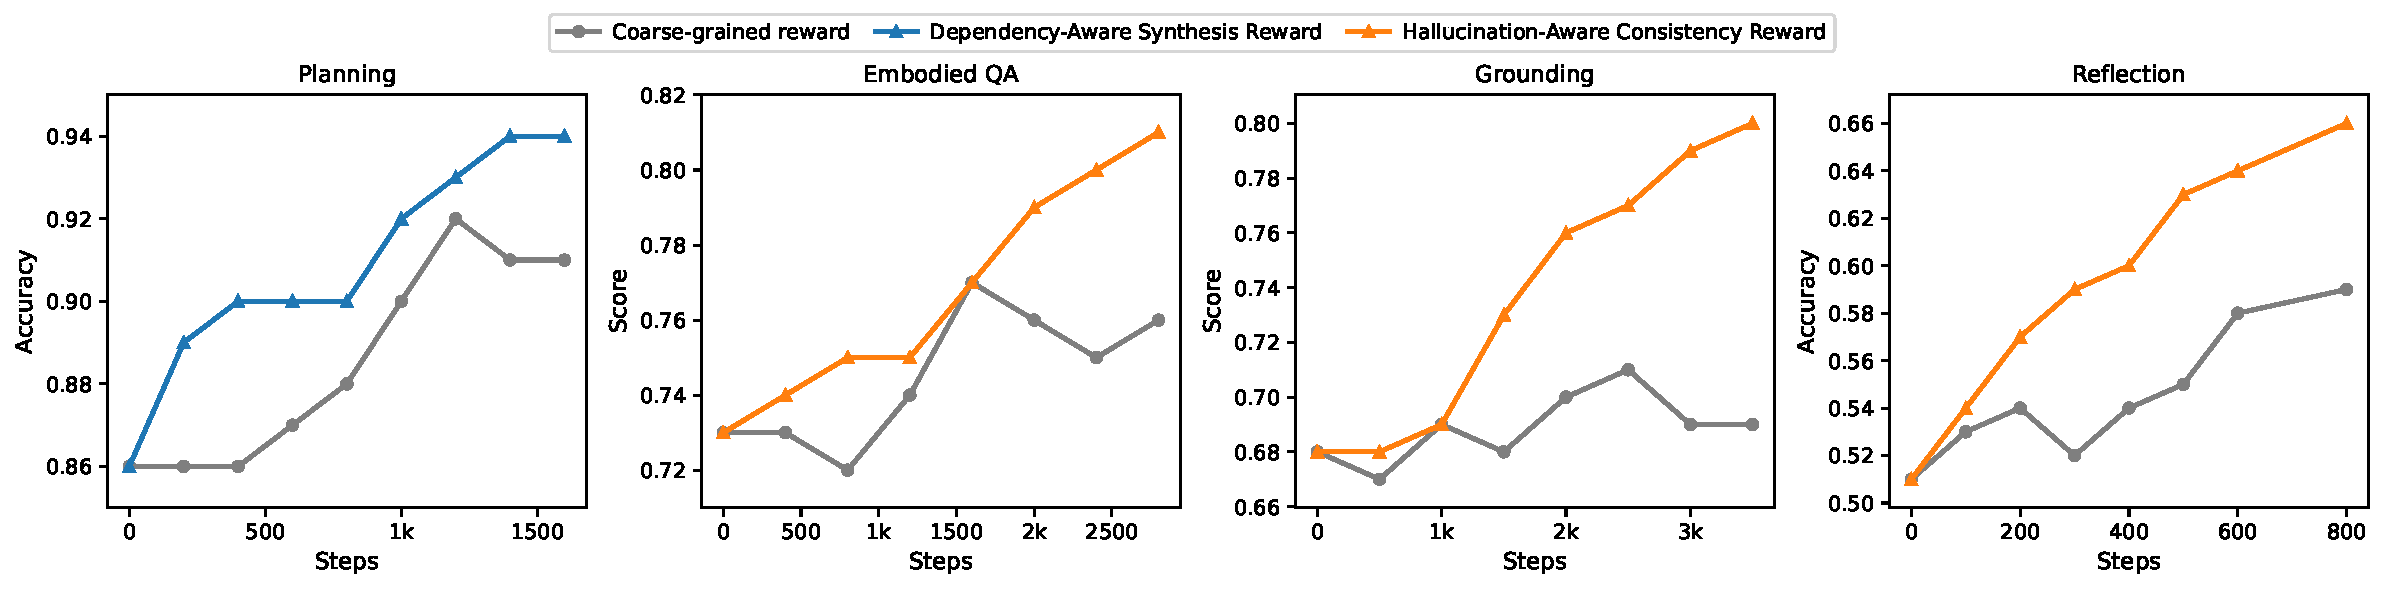
\includegraphics[width=1\textwidth]{figures/fig10.pdf}
\caption{Performance comparison between coarse-grained reward (GRPO) and our fine-grained rewards (DGRPO). Our Dependency-Aware Synthesis Reward and Hallucination-Aware Consistency Reward enable stable and consistent performance improvements, whereas using coarse-grained rewards leads to unstable RL training due to the lack of fine-grained supervision.
}
\label{fig:fig10}
\end{figure*}

\begin{table}[htbp]
\centering
\caption{
Ablation study of Optimus-3 on training stages. We report accuracy of Planning, Captioning, EQA, and Grounding on each stage.}
\label{tb:ablation_method}

\resizebox{0.48\textwidth}{!}{%
\begin{tabular}{ccc|cccc}
\toprule[1.2pt]
SFT & Coldstart & RL & Planning & Captioning & EQA & Grounding \\
\hline
          &           &           & 0.05 & 0.47 & 0.46 & 0.18 \\
\Checkmark &          &           & 0.79 & 0.68 & 0.71 & 0.52 \\
\Checkmark & \Checkmark &         & 0.86 & 0.72 & 0.73 & 0.68 \\
\Checkmark &          & \Checkmark & 0.76 & 0.71 & 0.68 & 0.79 \\


\rowcolor[HTML]{E7EEFE}
\Checkmark & \Checkmark & \Checkmark & \textbf{0.94} & \textbf{0.78} & \textbf{0.81} & \textbf{0.80} \\
\bottomrule[1.1pt]
\end{tabular}%
}
\end{table}
\texttt{CR} quantifies the agent's progress toward solving an open-ended task by measuring how many of the following stages it successfully completes in order: (1) Captioning, (2) Grounding, (3) Planning, (4) Action, and (5) Embodied QA. Formally, let $K$ denote the total number of stages and let $k_i$ be the number of stages completed in the $i$-th rollout. Given $N$ rollouts, the \texttt{CR} is defined as:
\begin{equation}
\texttt{CR} \;=\; \frac{1}{N}\sum_{i=1}^{N} \frac{k_i}{K}\;,
\end{equation}

\noindent\textbf{Baselines}. For the Open-ended Tasks, we compare Optimus-3 against generalist MLLMs (GPT-5 \cite{gpt4}, Qwen3-VL \cite{bai2025qwen2}, Gemini-2.5-pro \cite{team2024gemini}), and current SOTA agents in Minecraft (Jarvis-1 \cite{wang2023jarvis}, Optimus-1 \cite{li2024optimus}, and Optimus-2 \cite{li2025optimus}).


\noindent\textbf{Results Analysis}. As shown in Table~\ref{tb:main_open}, Optimus-3 achieves the highest task success rate and completion rate across all open-ended tasks. Notably, on the most challenging Diamond Sword task, Optimus-3 attains a success rate of 35\% and a completion rate of 69\%, demonstrating a substantial margin over all baselines. In contrast, generic MLLMs achieve consistently low success and completion rates on open-ended tasks, as they often fail to generate adaptive plans conditioned on the specific situation (e.g., the current inventory and surrounding environment). Meanwhile, even strong baselines such as Jarvis-1 \cite{wang2023jarvis} and Optimus-1 \cite{li2024optimus} struggle to generalize to open-ended settings. We attribute this to the fact that they are neither explicitly designed nor trained to support multi-dimensional abilities beyond planning and action execution. It highlights the advantage of Optimus-3: by integrating multi-dimensional capabilities into an end-to-end framework, it can better adapt to open-ended scenarios and solve tasks that require coherent perception--grounding--planning--execution--reflection loops.

\begin{figure*}[htbp]
    \centering
    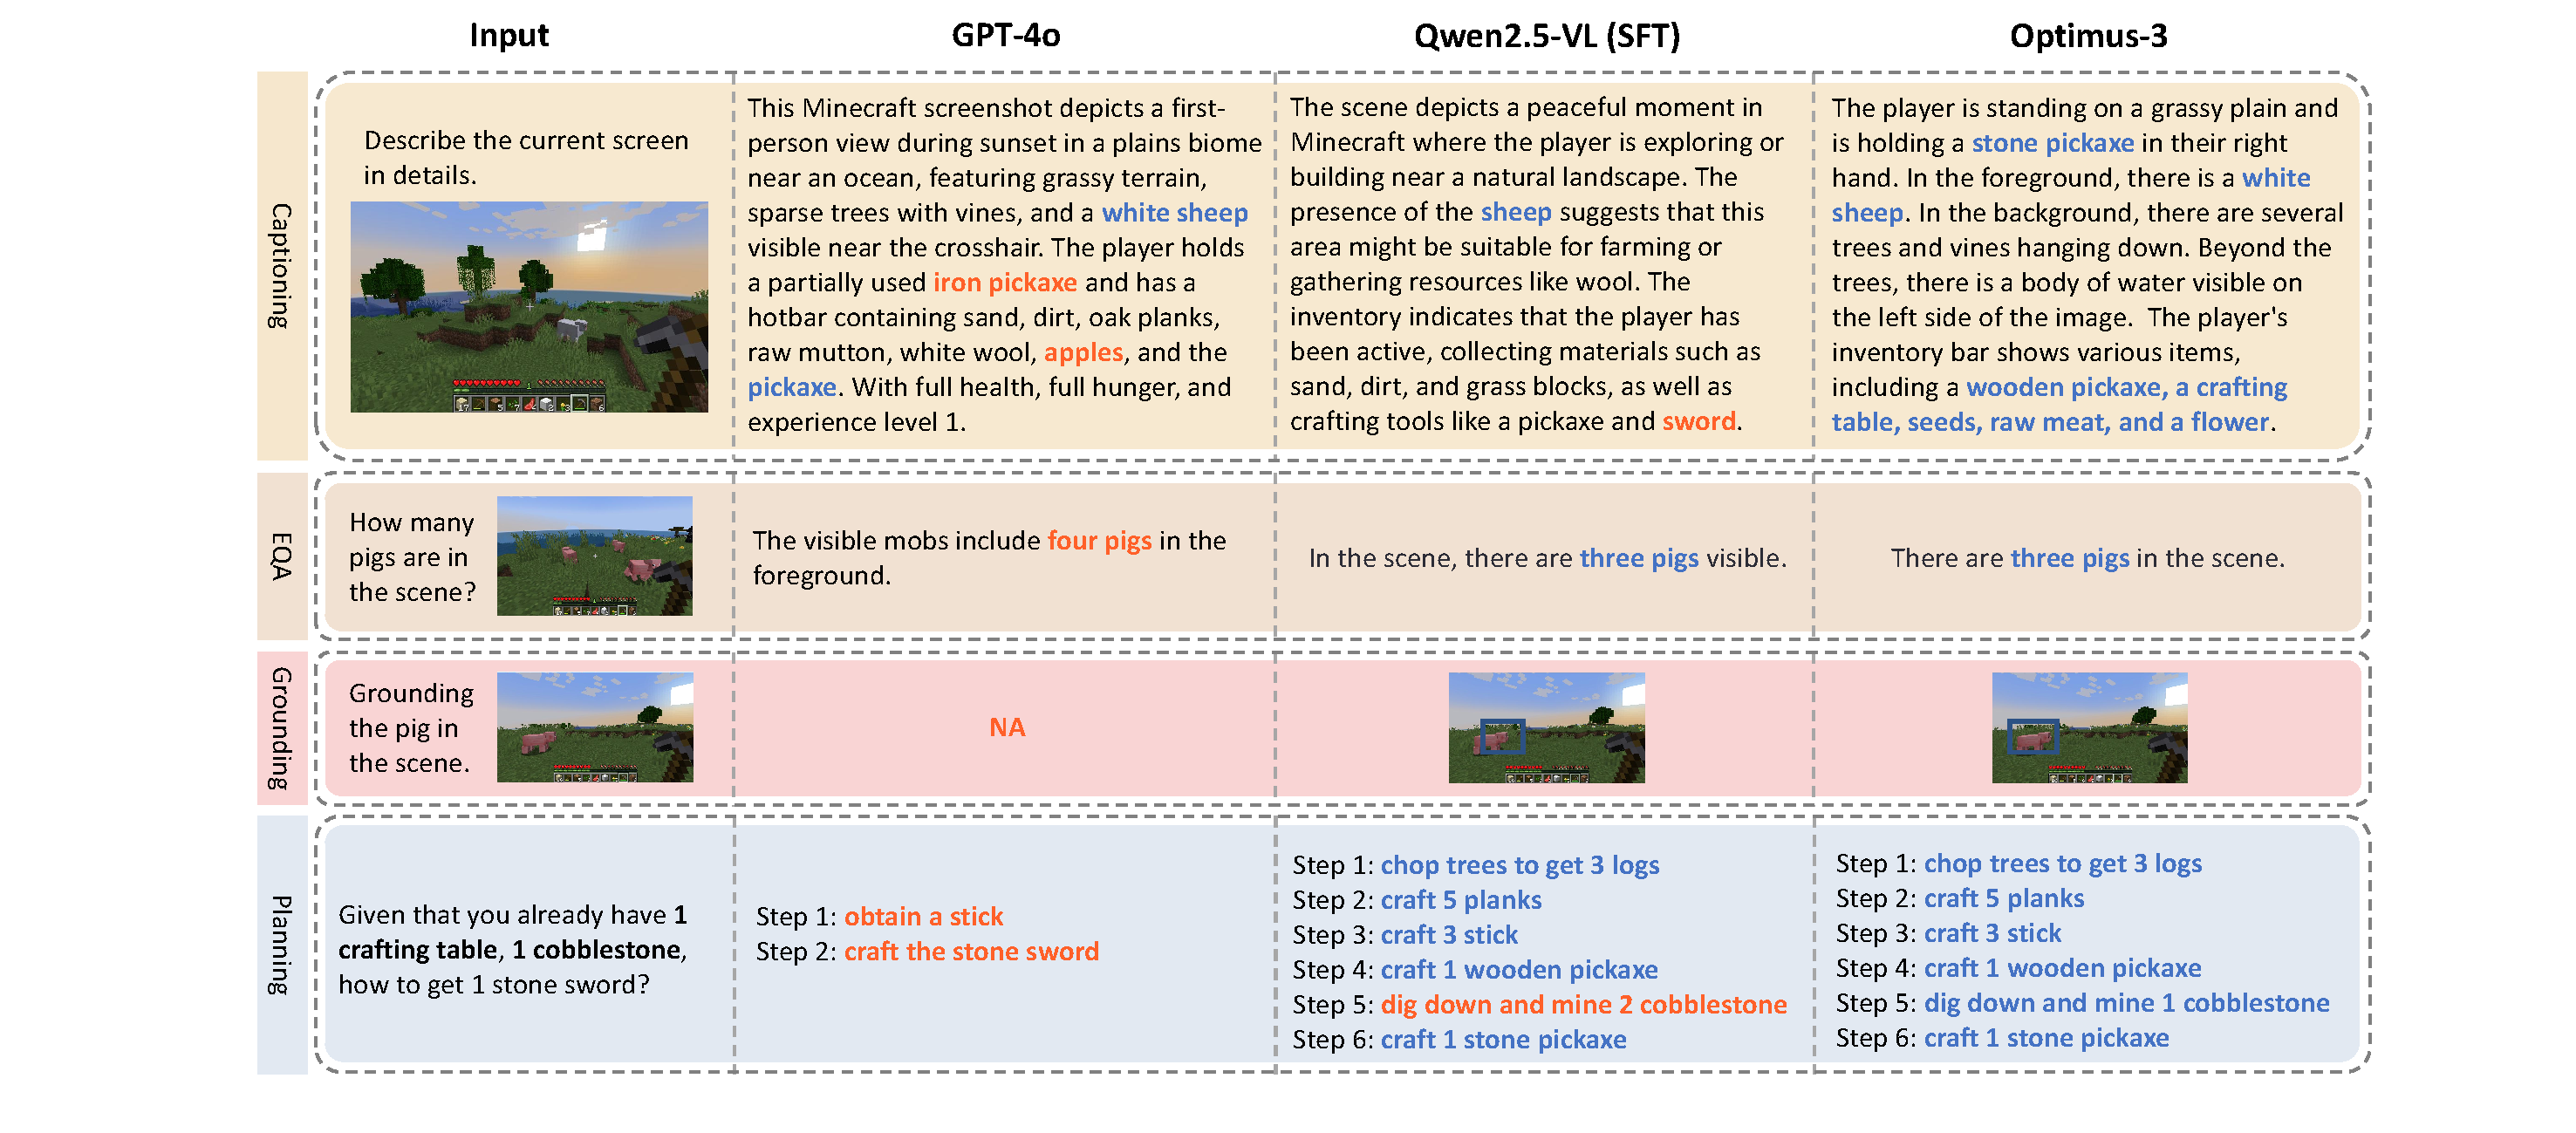
\includegraphics[width=1\textwidth]{figures/fig11.pdf}
    \caption{Visual comparison of Optimus-3 (ours), Qwen2.5-VL (tuned on our data), and GPT-4o. Red highlights indicate errors, while blue highlights denote correct outputs.}
    \label{fig:fig11}
\end{figure*}
\subsection{Ablation Study}
\label{ablation_study}
In this section, we conduct comprehensive ablation studies to validate the effectiveness of our approach and summarize our key findings.

\noindent\textbf{High-quality training data is essential for effective MLLM post-training}. Experimental results in Table \ref{tb:main_text} reveal that both Optimus-3 and \texttt{Qwen2.5-VL-SFT} benefit substantially from training on OptimusM$^4$ dataset. Furthermore, we conduct an ablation study to investigate the role of knowledge injection in our data-generation pipeline. As shown in Figure~\ref{fig:fig8}, removing the knowledge-augmentation mechanism (denoted as \texttt{Clear}) leads to substantial performance degradation, with drops of 81\% on Planning, 32\% on Embodied QA, and 23\% on Grounding, respectively. We attribute this degradation to the fact that generic MLLMs lack Minecraft-specific domain knowledge and thus produce low-quality synthetic data when the knowledge signal is removed. This result highlights the critical importance of our proposed knowledge-enhanced data generation pipeline in providing high-quality supervision for post-training the MLLM backbone. Moreover, the data collection process of OptimusM$^4$ incurred only \$300 in API costs, and was completed using 4$\times$ NVIDIA L40 GPUs over 36 hours, demonstrating the cost-efficiency of the pipeline.


\noindent\textbf{The Dual-Router Aligned MoE architecture is crucial for heterogeneous multi-task learning}. As shown in Table~\ref{tb:main_text}, dense models suffer from severe task interference when trained on heterogeneous multi-tasks, leading to suboptimal performance across all task types. Although the Optimus-3 variant with token routing outperforms the dense model on Planning and Embodied QA, it exhibits noticeable degradation on Captioning and Grounding. We attribute this behavior to the intrinsic difficulty of token-level routing, which must simultaneously address load balancing across experts and joint optimization over conflicting task objectives. In contrast, Optimus-3 with task routing achieves the best performance on all tasks. It indicates that explicitly assigning task-specific experts for heterogeneous tasks substantially mitigates task interference.



On the other hand, we conduct an ablation study to evaluate the impact of the Layer Router on latency-sensitive tasks, as illustrated in Figure~\ref{fig:fig9}. The results indicate that the Optimus-3 variant without the Layer Router suffers from an average per-action latency exceeding 50\,ms, thus failing to meet Minecraft's 20\,Hz interaction requirement. In contrast, introducing the Layer Router substantially accelerates the inference of Optimus-3 while preserving its high success rate. Remarkably, with the layer router enabled, the Optimus-3 with 6.8B parameters attains an inference speed comparable to Optimus-2 with 1.3B parameters. It highlights the role of the layer router in adapting the effective model depth to the task-dependent reasoning complexity. Taken together, these findings highlight the effectiveness of our proposed Dual-Router Aligned MoE architecture in simultaneously resolving conflicts among heterogeneous tasks and balancing inference complexity with real-time latency constraints.


\noindent\textbf{Dual-Granularity Reasoning-Aware Policy Optimization further enhances the agent’s capabilities}. As shown in Table \ref{tb:ablation_method}, removing the DGRPO method (both the \texttt{coldstart} and \texttt{RL} stages) leads to performance drops of 16\%, 13\%, 12\%, and 35\% on Planning, Captioning, EQA, and Grounding, respectively. These results highlight the pivotal role of DGRPO in enhancing the performance of Optimus-3 in dynamic and diverse scenarios. Furthermore, we conduct experiments to investigate the importance of our proposed fine-grained reward design. As shown in Figure~\ref{fig:fig10}, compared with using only the final answer correctness as a coarse feedback signal, our Dependency-Aware Synthesis Reward and Hallucination-Aware Consistency Reward yield consistently better performance on Planning, Embodied QA, Grounding, and Reflection. A critical ablation on the Embodied QA reveals that the model fails to converge when restricted to standard answer-level supervision. It shows the limitations of outcome-based RL in complex visual reasoning: the absence of process supervision renders the model vulnerable to visual hallucinations. In contrast, our DGRPO mitigates this issue by imposing strict penalties on non-existent entities generated within the reasoning chain. 

%These findings highlight the pivotal role of Process-Outcome Co-Supervision in the effective training of System 2 tasks.





\begin{figure*}[htbp]
    \centering
    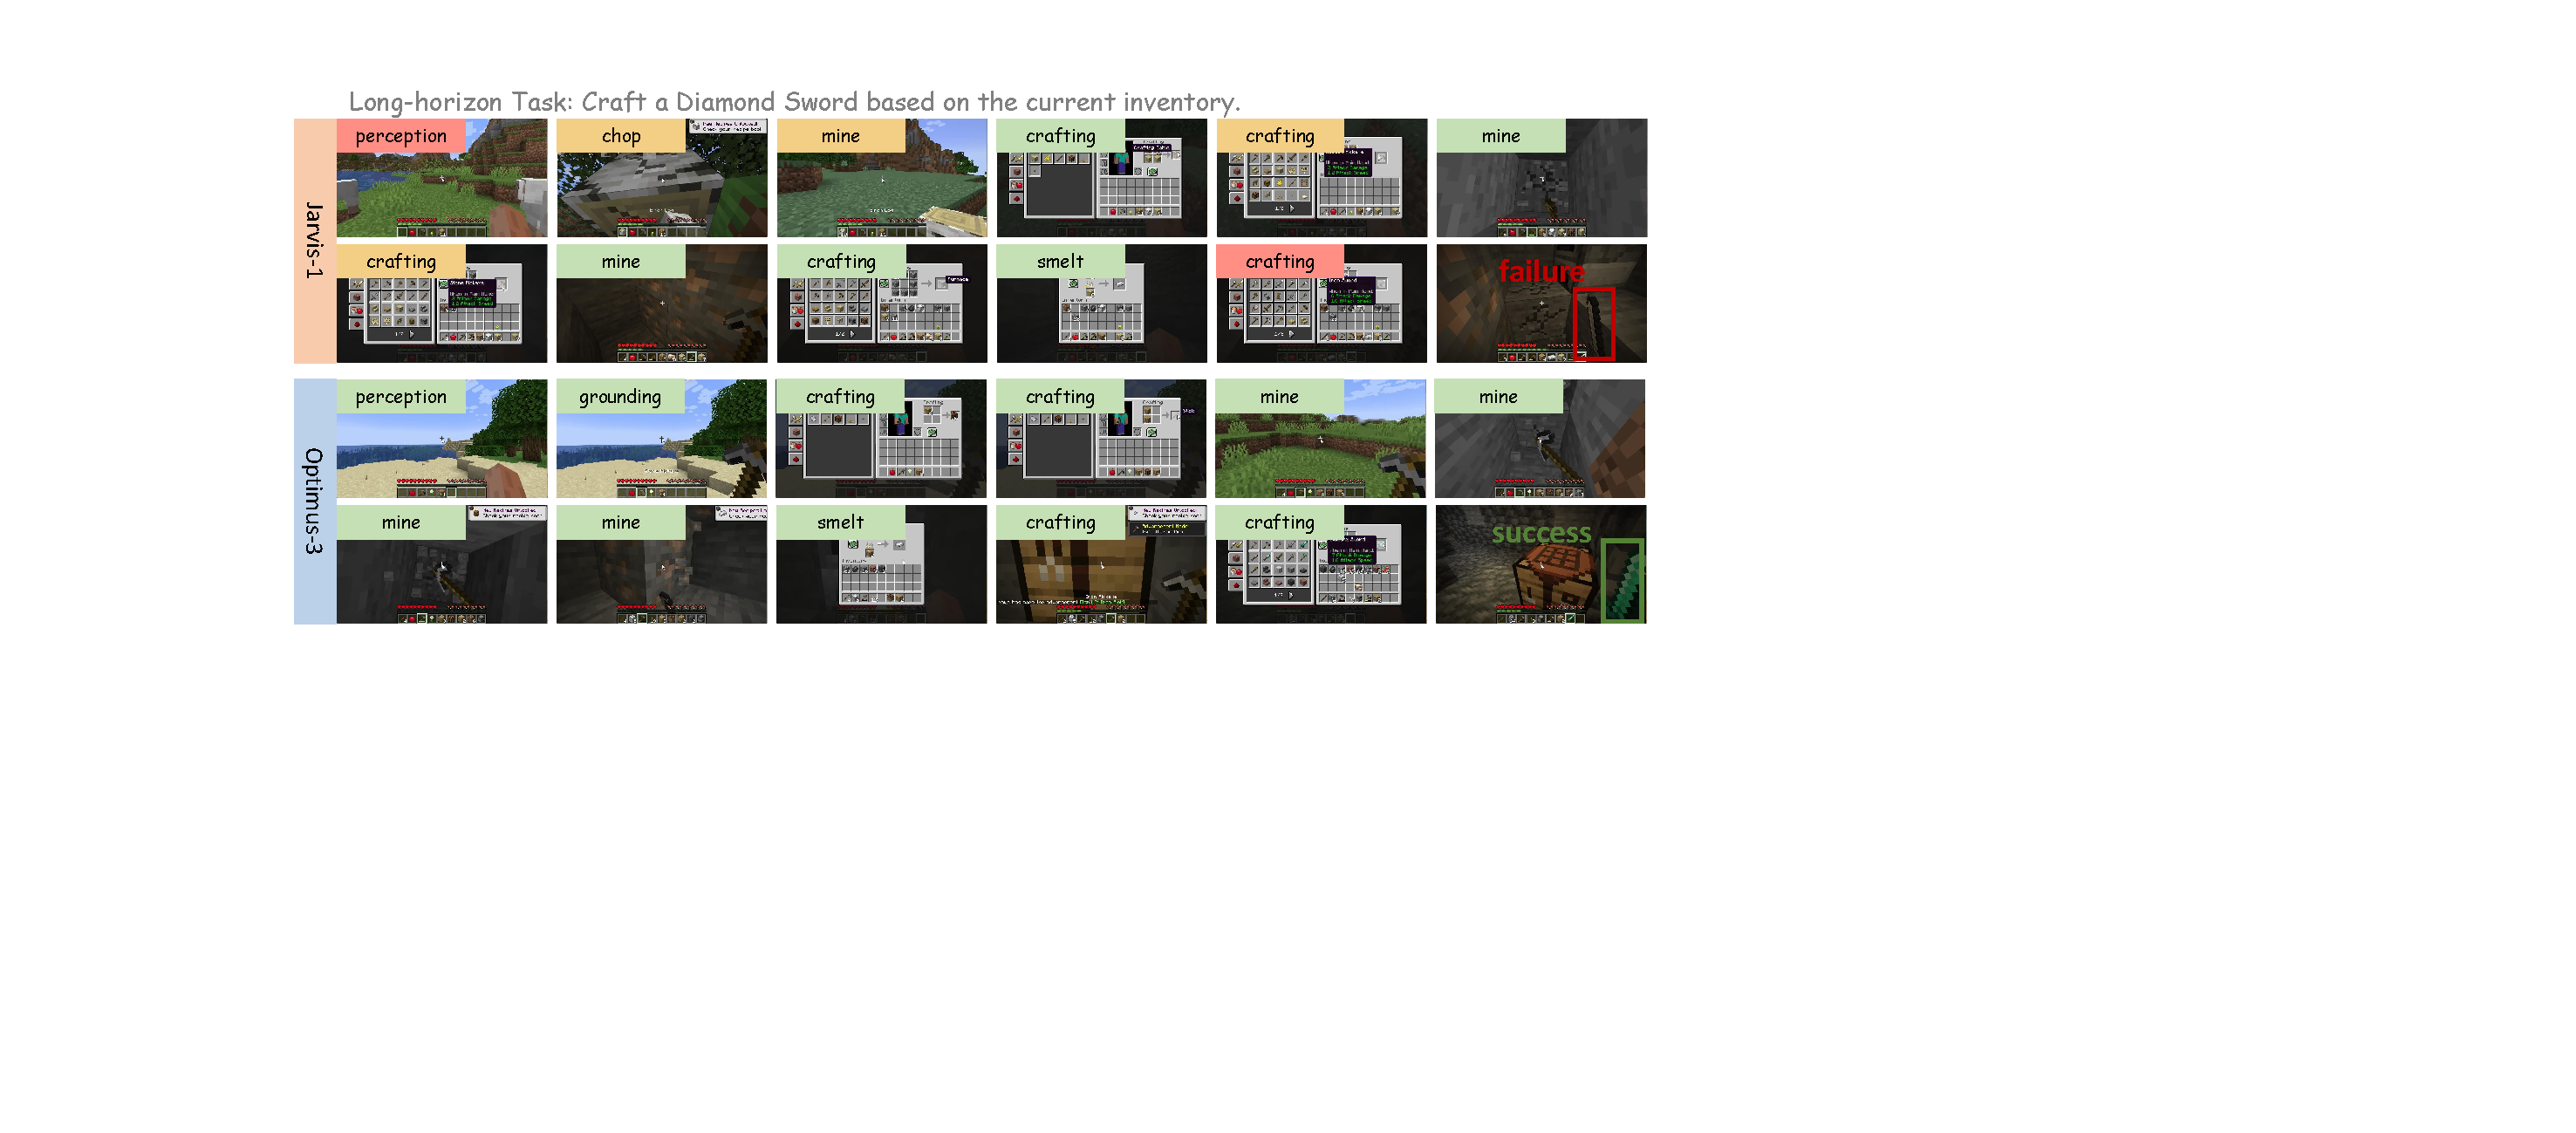
\includegraphics[width=1\textwidth]{figures/fig12.pdf}
    \caption{Visualization of Optimus-3 and Jarvis-1 executing the open-ended task \emph{``Craft a Diamond Sword based on the current inventory''}. Correct actions are highlighted in \colorbox{correct}{green}, unnecessary actions in \colorbox{unnec}{yellow}, and erroneous actions in \colorbox{wrong}{red}.}
    \label{fig:fig12}
\end{figure*}
\subsection{Qualitative Analysis} In this section, we present qualitative visualizations to illustrate the behavior of Optimus-3 across different task types. As depicted in Figure \ref{fig:fig11}, we provide a visual comparison between Optimus-3, Qwen2.5-VL-7B \cite{bai2025qwen2}, and GPT-4o \cite{gpt4}, highlighting their differences in performance and behavior across non-action tasks. We observe that GPT-4o exhibits hallucinations in captioning and embodied QA, lacks grounding capabilities, and produces unreasonable plans. In contrast, Qwen2.5-VL-SFT, which is fine-tuned on our OptimusM$^4$ dataset, shows reduced hallucination, acquires grounding and planning abilities, and generates more coherent outputs. Notably, Optimus-3 accurately performs vision-related tasks and produces well-structured plans conditioned on instructions, demonstrating its superior perception and reasoning in the Minecraft environment. 

Moreover, as shown in Figure~\ref{fig:fig12}, we compare Optimus-3 with Jarvis-1 \cite{wang2023jarvis} on the open-ended instruction, \textit{Craft a diamond sword based on the current inventory}. We observe that Jarvis-1 fails to accurately capture the fine-grained item information in the inventory (hotbar), which leads to planning trajectories containing unnecessary steps (e.g., crafting a Wooden Pickaxe 
\includegraphics[width=0.3cm]{figures/logo/wooden_pickaxe.pdf} and a Stone Pickaxe 
\includegraphics[width=0.3cm]{figures/logo/stone_pickaxe.pdf}). Moreover, the semantic gap between its planning and action modules causes it to eventually produce an incorrect target item. In contrast, Optimus-3 precisely understands the current context and generates an appropriate plan, successfully crafting the Diamond Sword 
\includegraphics[width=0.3cm]{figures/logo/diamond_sword.pdf} step-by-step. We attribute this performance to Optimus-3's integration of System 1 action loops and System 2 reasoning capabilities within a unified framework, which enables it adapts more effectively to the diverse situations encountered in Minecraft.



